% Template for ICASSP-2016 paper; to be used with:
%          spconf.sty  - ICASSP/ICIP LaTeX style file, and
%          IEEEbib.bst - IEEE bibliography style file.
% --------------------------------------------------------------------------
\documentclass{article}
\usepackage{spconf,amsmath,graphicx,float}

% Example definitions.
% --------------------
\def\x{{\mathbf x}}
\def\L{{\cal L}}

% Title.
% ------
\title{Comparison of Unsupervised Pre-training Methods}
%
% Single address.
% ---------------
\name{Jifu Zhao}
\address{University of Illinois at Urbana-Champaign\\
		 Department of Nuclear, Plasma, and Radiological Engineering\\
		 Urbana, Illinois 61801, USA}

\begin{document}
%\ninept
%
\maketitle

\section{Introduction}
\label{sec:intro}

As one important part of artificial intelligence (AI), machine learning has been widely used in our daily life, such as natural language processing (NLP), zip code recognition, self-driving cars and so on. Among those applications, supervised learning is the most common and perhaps the most powerful form of machine learning \cite{lecun2015deep}. For supervised learning, the choice of appropriate representations of original features is very important \cite{bengio2012deep}. For a long time, most machine learning applications require us to specify the input $\pmb{x}$ and target $\pmb{y}$. The choice of feature representation $\pmb{x}$ is usually determined by experts. However, sometimes the input $\pmb{x}$ may be just the raw feature without pre-processing. 

Researchers have been working on discovering the hidden structure of the data for years. In this process, several methods have been developed and found to be useful in some domains, such as Principal Component Analysis (PCA), Independent Component Analysis (ICA), Nonnegative Matrix Factorization (NMF), Restricted Boltzmann Machine (RBM), Auto-encoders and its variants and so on. These methods works in a unsupervised way and the output from these methods are thought to be a transformation of the raw input features. For supervised learning, some supervised learning mechanism will be built based on the output from these pre-training methods rather than the raw features. As expected, a good representation can help the supervised learning algorithms work better.

In this work, we focus on the comparison of several unsupervised per-training methods. More specifically, we will focus on PCA, kernel PCA and auto-encoders.

\section{Methods}
\label{sec:method}

\subsection{PCA}

Principal Component Analysis (PCA) is one of the most widely used pre-training methods for many applications. The goal of PCA is to find a lower dimensional linear space such that the variance of the orthogonal projection of the original data is maximized \cite{bishop2007pattern}. PCA is widely used for dimensionality reduction, feature extraction and data visualization. (Since this part has been covered in class, we won't cover too much derivations about PCA. Instead, we will focus on its application.)

\subsection{Kernel PCA}

As a linear transformation, PCA works well in some applications where the input data can be well represented by linear transformation. However, in a lot of applications, this assumption doesn't holds. We need some non-linear transformation for these scenarios. One direct idea is to map the input $\pmb{x}$ into some high dimensional space $\phi(\pmb{x})$ then perform PCA in this high dimensional. However, sometimes the dimensionality of the new space is so high that the computation PCA becomes very expensive. 

For this situation, Sch\"{o}lkopf \cite{scholkopf1998nonlinear, friedman2001elements} proposed the method called kernel PCA where the computation can be performed in the original feature space rather then the new space using so called kernel trick. In this way, through kernel PCA, a non-linear transformation makes it possible for us to find some complex representations. 

\subsection{Auto-encoders}

Auto-encoders use the input as the target, trying to find a reconstruction $r(x) = g(h(x))$ through so called encoder $h(\cdot)$ and decoder $g(\cdot)$ \cite{bengio2012deep}. In most cases, an auto-encoder is a multiple layer deep neural network which has a bottleneck structure. An 5 layer auto-encoder system is shown in Figure \ref{fig:autoencoder}.

\begin{figure}[htb]
\centering
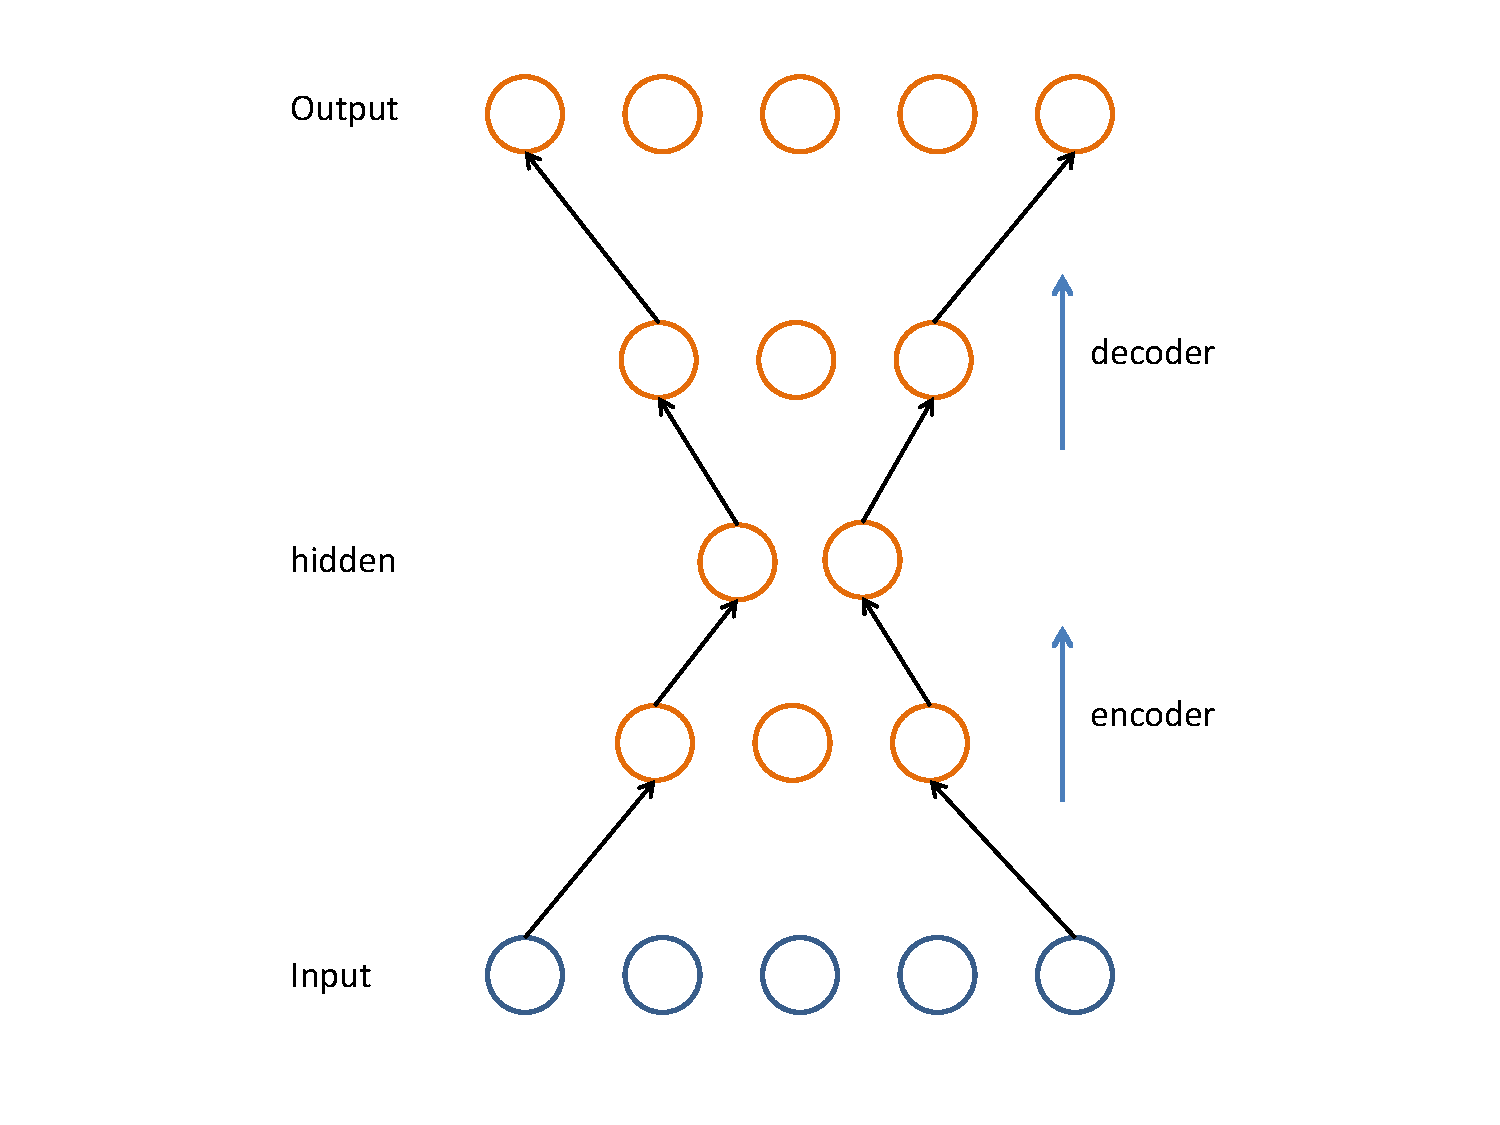
\includegraphics[width=8.5cm]{./figures/autoencoder.pdf}
\caption{Illustration of auto-encoder system.}
\label{fig:autoencoder}
\end{figure}

Auto-encoder system can be trained using back-prorogation methods. However, it works well only if we have a good initialization for the auto-encoder systems \cite{hinton2006reducing}. Hinton and Salakhutdinov \cite{hinton2006reducing} then proposed an effective way of initialization which utilize a stack of RBMs for pre-training. After unrolling, the whole auto-encoder system can be fine-tuned.

\section{Data}
\label{sec:data}

In this work, we plan to use the MNIST dataset \cite{lecun1998gradient}. The MNIST dataset contains a huge amount of handwirtten digits. It has $60000$ training examples (more precisely, $55000$ training examples, $5000$ validation examples) and $10000$ test examples. It has $10$ classes which corresponding to digits from $0$ to $9$. Each example is a $28 \times 28$ pixel grayscale image. The pixel values range from $0$ to $1$. A subset of $36$ examples is shown in Figure \ref{fig:filter}.

\begin{figure}[htb]
\centering
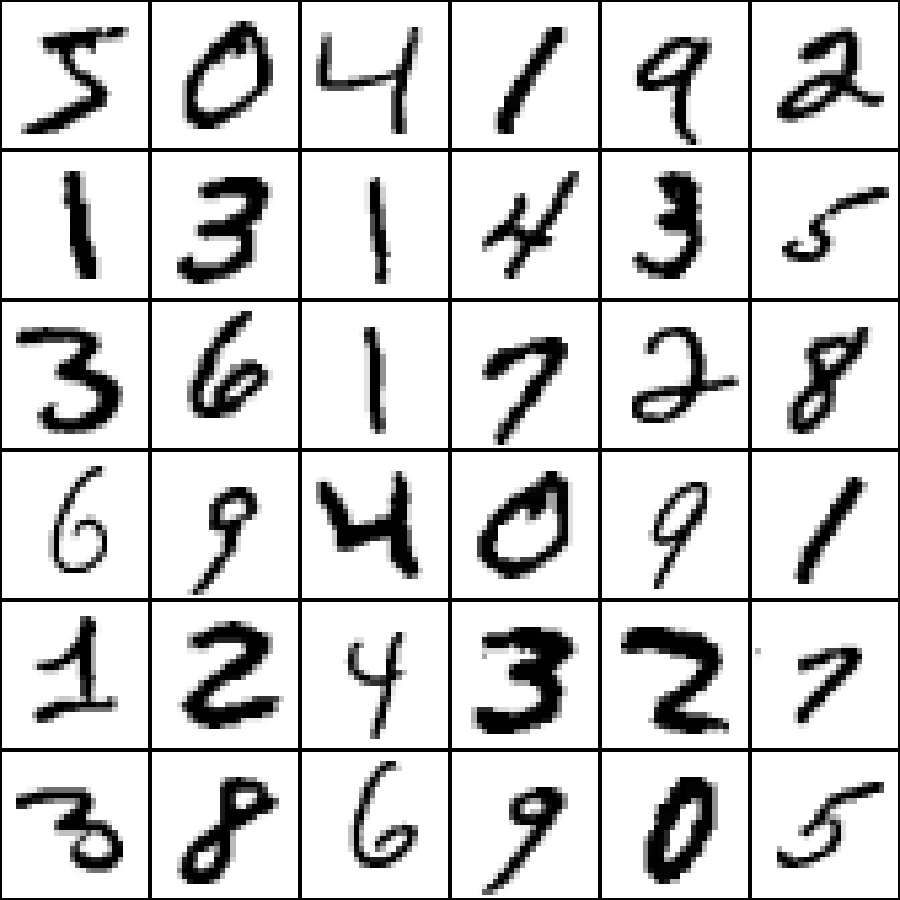
\includegraphics[width=8.5cm]{./figures/filter.pdf}
\caption{Examples of MNIST dataset.}
\label{fig:filter}
\end{figure}

\section{Experiments}
\label{sec:experiment}

This work is an extension of the assignment 4, where we are required to compare the classification accuracy for raw image, PCA, RBM and stacked RBMs. In this work, we will use similar procedure, but focus on kernel PCA and auto-encoder systems.

Our work can be roughly divided into two parts. The first part will be focused on the comparison of PCA and kernel PCA. More specifically, we will conduct experiments on PCA and kernel PCA with polynomial kernel and rbf kernel. Through choosing different number of transformed features, we will build a supervised multiclass classifier to classify the dataset into $10$ classes. Through calculating the error rate of different methods, we hope to compare the performance of different methods.

The second part will focused on the auto-encoders. Except the study on number of hidden nodes and number of layers, we will also study the influence of pre-training using stacks of RBMs as described by Hinton and Salakhutdinov \cite{hinton2006reducing}. Then the same classification strategy will be implemented.

Since the goal of this work is to study different pre-training methods, the final classifier won't be very complicated, a multiclass Support Vector Machine (SVM) or a two-layer multi-class logistic regression neural network will be used.

\section{Resource Feasibility}
\label{sec:feasibility}

With a modern computer (i.e., Intel i$7$ processor, $16$ RAM), most of the work described above can be implemented without any problem. However, for kernel PCA part, the kernel matrix $K$ has the dimensionality of $n \times n$, where n is the number of given samples. In this work, for the MNIST dataset, there will be $60000$ training examples. The dimensionality of $K$ will be $60000 \times 60000$. To store this matrix in memory, it will need more than $25$ GB (using numpy.float64 data type), which is not possible for our current computer. For this part, we will implement the algorithm on Amazon Web Service (AWS).

\section{Timeline}
\label{sec:timeline}

We expect to finish the theoretical derivation part before the Thanksgiving. Then focus on actual programming part after the Thanksgiving ($11/24/2016$). For programming part, we will implement kernel PCA through Python3 + Numpy. For auto-encoder part, we will implement it through TensorFlow + TFLearn. We expect the conduct the actual experiment part from $11/28/2016$ and finish all parts before $12/07/2016$.

\vfill\pagebreak

% References should be produced using the bibtex program from suitable
% BiBTeX files (here: strings, refs, manuals). The IEEEbib.bst bibliography
% style file from IEEE produces unsorted bibliography list.
% -------------------------------------------------------------------------
\bibliographystyle{IEEEbib}
%\bibliography{strings,refs}
\bibliography{strings}

\end{document}
